\section{Request handling}

\begin{frame}[t]{What is request handling?}

	\note{Τι είναι η διαχείριση των αιτημάτων ενός VM?\\
		Είναι η εφαρμογή πολιτικών και επεξεργασία των αιτημάτων σε όλη 
		την πορεία τους μέχρι το να φτάσουν στο storage.\dspc
		Δηλαδή έχουμε ένα εικονικό μηχάνημα <κλικ>\\
		... το storage μας <κλικ>\\
		και πρέπει με κάποιο τρόπο τα δεδομένα του μηχανήματος να 
		φτάσουν σε εμάς <κλικ>\\

		Ένας απλός τρόπος θα ήταν να τα συνδέσουμε. Άλλωστε όταν τρέχει 
		VM, ο hypervisor κοιτάει block device. Θα μπορούσε να ήταν 
		κομμάτι του storage
		Είναι αυτό αρκετό; <κλικ>\\
		Όχι, χρειαζόμαστε επίσης \fixme
	}


	\begin{columns}[t]
		\begin{column}{.5\textwidth}
			\pause
			\makebox[\textwidth]{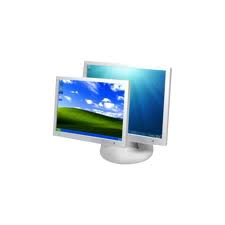
\includegraphics[width=.2\paperwidth]{images/vm.jpg}}
			\pause \centering{ {\Huge +} }
				\makebox[\textwidth]{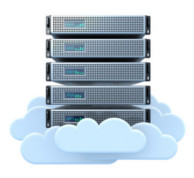
\includegraphics[width=.2\paperwidth]{images/cloud-server1.jpg}}
			\pause \centering{ {\Huge = ?}}
		\end{column}
		\begin{column}{.5\textwidth}
			\pause
			\begin{itemize}
				\item Policy enforcement?
				\item Storage agnosticity?
			\end{itemize}
		\end{column}
	\end{columns}

\end{frame}

\begin{frame}{Our solution}

	{\Large Archipelago}

	\makebox[\textwidth]{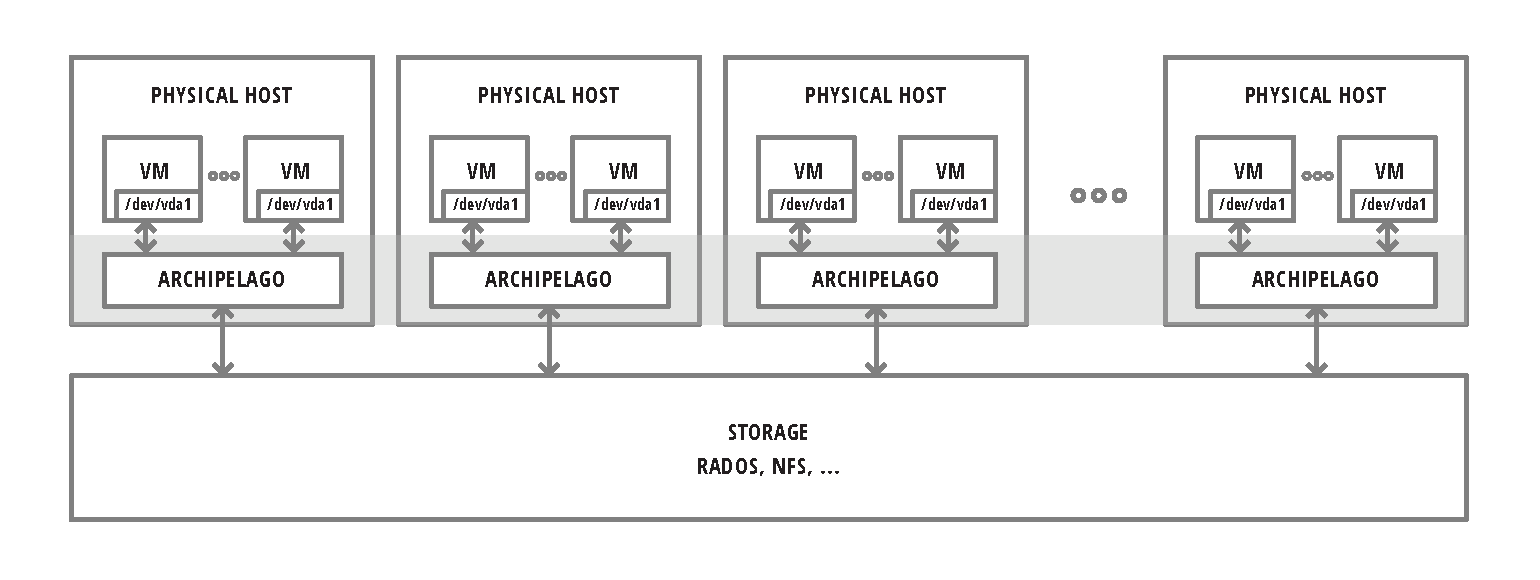
\includegraphics[width=\textwidth]{images/archipelago_overview_a.pdf}}

	\spc

	Key features:
		1) Software-defined
		2) Distributed
		) Modular
		Copy-On-Write
		Storage agnostic

	\note{Η λύση που χρησιμοποιήσαμε είναι το Archipelago}
	\note{
		\begin{itemize}
			\item Software-defined: αν και είναι ένα όρος 
				μαρκετινγκ, εμείς κανονικά. Σημαίνει με το 
				software ΟΡΙΖΕΙΣ το storage (εφαρμογή policy, 
				αλλαγή πορείας του request)
			\item τρέχει σε πολλούς κόμβους
			\item αποτελείται από διακριτά κομμάτια
			\item κάνει CoW (εξήγησε ότι τα images είναι λίγα, τα
				VMs πολλά, όπως όταν ένα process κάνει fork)
			\item μπορούμε χρησιμοποιήσουμε ότι θέλουμε
		\end{itemize}
	}

\end{frame}

\begin{frame}{Archipelago Architecture}
	%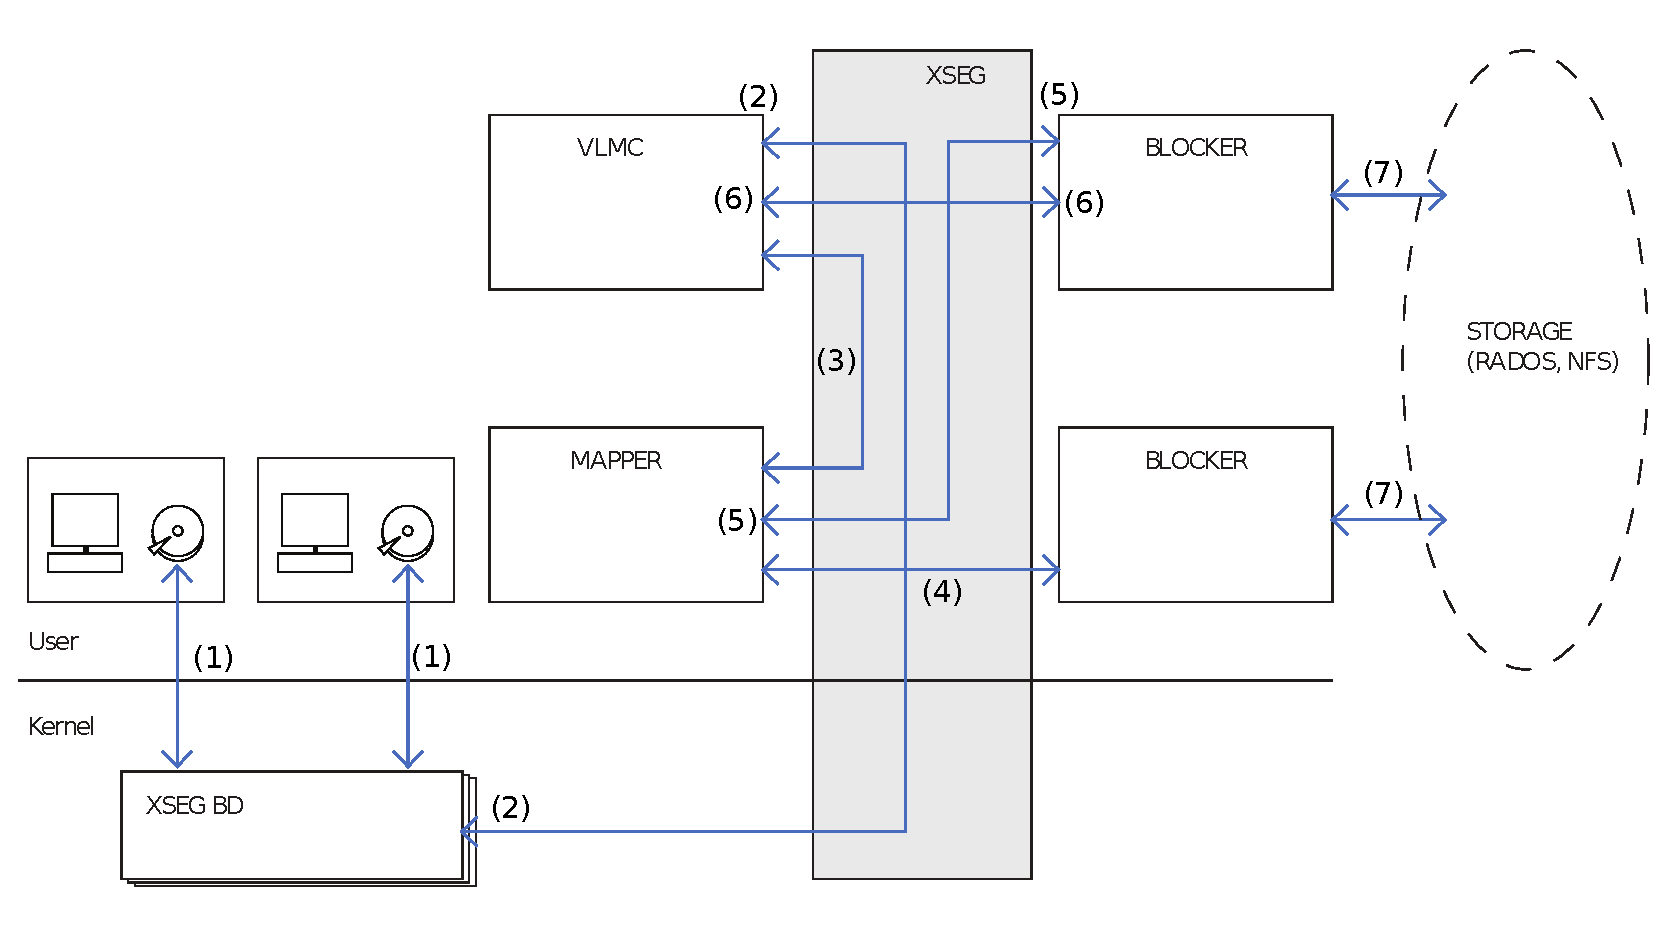
\includegraphics[{images/new_sxima_numbered.pdf}
	\begin{center}
		  \makebox[\textwidth]{\includegraphics[width=0.9\paperwidth]{images/new_sxima_numbered.pdf}}
	\end{center}

	\note{
		\begin{itemize}
			\item To VM στέλνει αίτημα στο δίσκο του, ο δίσκος 
				είναι εικονικός, θα το δει ο hypervisor 
				(εξήγησε τι είναι ο hypervisor) και θα το 
				στείλει στον δίσκο που το έχουμε πει. (xsegbd)
			\item 2) \fixme 
		\end{itemize}
	}
			
\end{frame}

\begin{frame}{RADOS}

	The object store component of Ceph filesystem.\\
	\spc
	Key features:
	\begin{itemize}
		\item Replication
		\item Fault tolerance
		\item Self-management
		\item Scalability
	\end{itemize}


	\pause

	\spc
	Speed issues:\\
	VM with page-cache: > 90MB/s, < 1ms\\
	VM without page-cache: < 7MB/s, ~ 10ms

	\pause

	\spc
	Thesis goal: make this faster.

\end{frame}

